% Chapter sectioning
\hypertarget{appendix}{%
\section{Appendix}\label{appendix}}

\hypertarget{new-functions-that-come-with-tribunal}{%
\subsection{New functions that come with
TRIBUNAL}\label{new-functions-that-come-with-tribunal}}

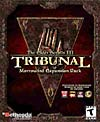
\includegraphics{media/image6.png} The Tribunal expansion for Morrowind
introduced a number of new functions and fixes and extends several of
the old ones. Note that both you and the user of the mod must have
Tribunal (or Bloodmoon, or GOTY edition) installed to make use of these,
so make sure you mark your mod accordingly. The functions are now sorted
into the main document, but this list may serve as an easy reference to
see which functions are Tribunal functions.

(Many thanks to Bethsoft's Mike Lipari for sharing the information on
these functions with the community.)

\hypertarget{changes-fixes-to-morrowind-scripting}{%
\subsubsection{Changes / fixes to Morrowind
scripting:}\label{changes-fixes-to-morrowind-scripting}}

\begin{itemize}
\item
  SetPos now accepts variables (float) as arguments.
\item
  SetAngle now accepts variables (float) as arguments.
\item
  Equip now works as intended and forces NPC to equip (put on) armor and
  clothing.
\item
  AIActivate was apparently fixed.
\end{itemize}

\hypertarget{index-of-new-tribunal-script-functions}{%
\subsubsection{Index of new Tribunal Script
Functions:}\label{index-of-new-tribunal-script-functions}}

%\hypertarget{section-13}{%
%\subsubsection{}\label{section-13}}

AddToLevCreature

AddToLevItem

ClearForceJump

ClearForceMoveJump

ClearForceRun

DaysPassed (variable)

DisableLevitation

EnableLevitation

ExplodeSpell

ForceJump

ForceMoveJump

ForceRun

GetArmorType

GetCollidingActor

GetCollidingPC

GetForceJump

GetForceMoveJump

GetForceRun

GetPCJumping

GetPCRunning

GetPCSneaking

GetScale

GetSpellReadied

GetSquareRoot

GetWaterLevel

GetWeaponDrawn

GetWeaponType

HasItemEquipped

HurtCollidingActor

ModScale

ModWaterLevel

PlaceItem

RemoveFromLevCreature

RemoveFromLevItem

SetDelete

SetJournalIndex (?)

SetScale

SetWaterLevel

\hypertarget{new-functions-that-come-with-bloodmoon}{%
\subsection{New functions that come with
BLOODMOON}\label{new-functions-that-come-with-bloodmoon}}

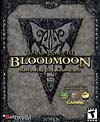
\includegraphics{media/image7.png} The second expansion for Morrowind,
Bloodmoon, introduces a few new functions. Note that both you and the
user of the mod must have Bloodmoon installed to make use of these, so
make sure you mark your mod accordingly.

\hypertarget{index-of-new-bloodmoon-script-functions-and-variables}{%
\subsubsection{Index of new Bloodmoon Script Functions and
variables:}\label{index-of-new-bloodmoon-script-functions-and-variables}}

AllowWereWolfForceGreeting

BecomeWerewolf

GetPCInJail

GetPCTraveling

GetWerewolfKills

IsWerewolf

PCKnownWerewolf

PlaceAtMe

SetWerewolfAcrobatics

TurnMoonRed

TurnMoonWhite

UndoWerewolf

\hypertarget{previously-undocumented-functions}{%
\subsection{\texorpdfstring{\hfill\break
Previously undocumented
functions}{ Previously undocumented functions}}\label{previously-undocumented-functions}}

These functions were not documented in the original helpfile. I have
explained most of them in this guide, but for a few the uses are still
unknown to me. I thought it might be useful to have as a list for an
easy overview. The list was put together by someone who Hex-edited the
TES-CS .exe, so it's likely to be complete.

(thanks to Soralis for the list and XPCagey and others who helped to put
it together):

\textbf{Undocumented in Helpfile:}

PayFineThief

EnableStatReviewMenu

GetFactionReaction

ShowMap

EnableBirthMenu

EnableClassMenu

EnableRaceMenu

EnableNameMenu

RemoveEffects

EnableMagicMenu

EnableMapMenu

EnableInventoryMenu

EnableStatsMenu

GetInterior

GetLineOfSight (alias for GetLOS)

GetWindSpeed

GetCurrentTime

ResetActors

OutputRefInfo

MenuTest

Functions which are \textbf{spelled differently than documented
(XPCagey):}

getHealthRatio -> getHealthGetRatio

getInvisible -> getInvisibile

setInvisible -> setInvisibile

modInvisible -> modInvisibile

getSecundusPhase -> getSecundaPhase

\textbf{(actual syntax on the right)}

And those which don't work:

getPlayerViewSwitch -> (can't be used)

OnRepair -> not in string tables

UsedOnMe -> not in string tables

name -> not in string tables

Also be aware that most console commands can be compiled as functions by
the Construction Set (see list below). These are also to a large part
not listed by the helpfile.

\hypertarget{variable-type-functions}{%
\subsection{\texorpdfstring{\hfill\break
Variable-type
functions:}{ Variable-type functions:}}\label{variable-type-functions}}

For easy reference, the following list shows all those variable/function
type hybrids that you \textbf{need to declare} as variables if you use
them in a script.

\hypertarget{local-variables-that-get-set-by-the-game}{%
\subsubsection{Local variables that get set by the
game:}\label{local-variables-that-get-set-by-the-game}}

Short OnPCEquip

Short OnPCAdd

Short OnPCRepair

Short OnPCSoulGemUse

Short OnPCHitMe

Float minimumProfit (Tribunal)

\hypertarget{local-variables-that-you-can-set-as-a-flag}{%
\subsubsection{Local variables that you can set as a
flag:}\label{local-variables-that-you-can-set-as-a-flag}}

Short Companion (Tribunal)

Short StayOutside (Tribunal)

Short PCSkipEquip

\hypertarget{special-globals}{%
\subsubsection{Special Globals}\label{special-globals}}

Some globals hold special significance that you can take advantage of
for your own scripting. Since they are globals, you do not need to
declare them.

\begin{longtable}[]{@{}
  >{\raggedright\arraybackslash}p{(\columnwidth - 2\tabcolsep) * \real{0.36}}
  >{\raggedright\arraybackslash}p{(\columnwidth - 2\tabcolsep) * \real{0.64}}@{}}
\toprule
\endhead
Short NPCVoiceDistance (750) & Used as a distance when Following NPCs
call after you to wait for them (e.g. see DandsaScript) \\
Float GameHour & Holds the current hour of the day (0-23)

Note, this is a float, so 10:30 would be represented as 10.5. See the
section on float variables for more information \\
Short Day & Holds the current day of the month (1-30) \\
Short Month & Holds the current Month of the year (0-11) \\
Short Year (427) & Holds the current year \\
Float TimeScale (30) & Sets the ratio of real-time/game-time \\
Short Random100 & Is randomly set between 0-100 (set by main script when
out of menumode) \\
Short PCRace & Contains the player's Race

(1=Argonian, 2=Breton, 3=Dark Elf, 4=High Elf, 5=Imperial, 6= Khajiit,
7=Nord, 8=Orc, 9=Redguard, 10=Woodelf)

If the player is using a custom race, PCRace will remain 0 by default.
Note that it is possible to add your own racecheck script for custom
races, and set PCRace to a custom value, but be warned: if two mods do
this, you may have conflicts. As this variable is only used in dialog,
it is not required that you set it to a different number for every
custom race you make. If you made a new race with dialog, instead of
using this it would be far better to make your own global variable as it
would be less likely to conflict with other mods. \\
Short PCVampire & Vampire status: 0=Normal, 1=Vampire, -1= cured \\
Short VampClan & If the PC becomes a vampire, this indicates his clan.
1=Aundae, 2=Berne, 3=Quarra \\
Short DaysPassed & Contains the number of days since the game started.
Requires an explicit declaration, which is present in Tribunal but must
otherwise be added (not present in Bloodmoon or Morrowind). \\
Short PCWerewolf & Werewolf status: 0=Normal, 1=Werewolf, -1=Cured \\
Float WerewolfClawMult (25.00) & Increased during the Werewolf quests to
make your claw attack more powerful. \\
Short PCHasGoldDiscount & Used in dialogue. Gets set to 1 if player has
enough gold to pay thieves guild discount on the "price on your
head". \\
Short PCHAsTurnIn & Used in dialogue. Gets set to 1 if player has enough
gold to pay the reduced fee for turning yourself in. \\
Short PCHasCrimeGold & Used in dialogue. Gets set to 1 if player has
enough gold to pay the crime fee. \\
Short CrimeGoldTurnIn & Gold needed for reduced crime fee \\
CrimeGoldDiscount & Gold needed for thieves guild discount crime fee \\
\bottomrule
\end{longtable}

\hypertarget{game-units}{%
\subsection{\texorpdfstring{\hfill\break
Game units:}{ Game units:}}\label{game-units}}

1 game unit = 0.56 inches\\
50 =28 inches\\
500 = 23.3 feet\\
5000 = 233.3 feet\\
8192 = 385 feet = 1 game cell

1 game unit = 1.42 cm\\
100 game units = 142 cm = 1.42 meters\\
1000 game units = 14.2 meters\\
8192 game units = 116.33 meters = 1 exterior cell

The island of Morrowind itself is 5.00 km north to south and 4.65 km
east to west.

(thanks to Iudas for this information)

\hypertarget{derived-attribute-calculations}{%
\subsection{Derived attribute
calculations:}\label{derived-attribute-calculations}}

(Thanks to DinkumThinkum for this info.)

The following is based on how they're calculated for player characters;
checking in the Construction Set, NPC derived attributes appear to use
basically the same system (if auto-calculate is enabled).

\textbf{Maximum Fatigue:} equals the total of current Strength, current
Endurance, current Willpower, and current Agility.

\textbf{Maximum Magicka:} current Intelligence times the character's
magicka multiplier (varies with race and birthsign). For NPCs, the
multiplier apparently is fixed at two (default value of
fNPCbaseMagickaMult: see Game Settings); race doesn't seem to affect it.

NOTE: this is based on the Maximum Magicka shown in the editor. Racial
abilities that fortify Maximum Magicka are listed in the 'spells'
section of the NPC's properties page, so that may be figured into the
maximum value used during game play; haven't tested this.

\textbf{Maximum Encumbrance:} five times the character's current
Strength.

\textbf{Maximum Health (player):} When you create your character, their
starting maximum Health (at first level) is one half the total of their
Strength and Endurance. After that, each time your character goes up a
level their maximum Health is increased by 10\% of their Endurance
(value set by fLevelUpHealthEndMult, see Game Settings). This is based
on the character's base natural Endurance; magical modifications to
Endurance are ignored.

Strength is only used to calculate the player character's starting value
for maximum Health; it has no further affect on Health once the
character has been created. Also, Endurance affects the amount added to
the character's maximum Health each level; there's no recalculation of
the amount added in previous levels.

\textbf{Maximum Health (NPCs):} A number of formulas for NPC health have
been proposed, but I (melian) have yet to find one that works for more
than one NPC. At base level, NPC Health appears to be auto-calculated in
the same way as the player's: (STR + END)/2. After that it gets tricky,
and most formulas fail quite dramatically at higher levels.

For \emph{some} NPCs: The calculation is based on the character's
Strength and Endurance, and Health increase factor per level is constant
within three brackets: before STR has maxed (largest increase), after
STR but before END has maxed (smaller increase), and after both have
maxed (constant smaller increase from then on). It's usually easy enough
to calculate a single NPC's Health at any given level by noting Health,
Strength and Endurance at various levels and working out the increase
factor per level in each of the three brackets (remembering that values
are really floats: averaging a larger value will get a more accurate
increase factor). This has worked for most NPCs I've used it on, whose
Strength maxed well before Endurance did. I'm not sure of the
progression for NPCs whose Endurance maxes first, and race may have
something to do with it as well.\protect\hypertarget{_Toc53412751}{}{}

\hypertarget{magic-effect-list}{%
\subsection{Magic Effect List}\label{magic-effect-list}}

For the function GetEffect, you need the ID-string itself (e.g.
GetEffect sEffectWaterBreathing). For the RemoveEffects function, the
effect number is used (e.g. RemoveEffects, 0)

0 => sEffectWaterBreathing\\
1 => sEffectSwiftSwim\\
2 => sEffectWaterWalking\\
3 => sEffectShield\\
4 => sEffectFireShield\\
5 => sEffectLightningShield\\
6 => sEffectFrostShield\\
7 => sEffectBurden\\
8 => sEffectFeather\\
9 => sEffectJump\\
10 => sEffectLevitate\\
11 => sEffectSlowFall\\
12 => sEffectLock\\
13 => sEffectOpen\\
14 => sEffectFireDamage\\
15 => sEffectShockDamage\\
16 => sEffectFrostDamage\\
17 => sEffectDrainAttribute\\
18 => sEffectDrainHealth\\
19 => sEffectDrainSpellpoints\\
20 => sEffectDrainFatigue\\
21 => sEffectDrainSkill\\
22 => sEffectDamageAttribute\\
23 => sEffectDamageHealth\\
24 => sEffectDamageMagicka\\
25 => sEffectDamageFatigue\\
26 => sEffectDamageSkill\\
27 => sEffectPoison\\
28 => sEffectWeaknessToFire\\
29 => sEffectWeaknessToFrost\\
30 => sEffectWeaknessToShock\\
31 => sEffectWeaknessToMagicka\\
32 => sEffectWeaknessToCommonDisease\\
33 => sEffectWeaknessToBlightDisease\\
34 => sEffectWeaknessToCorprusDisease\\
35 => sEffectWeaknessToPoison\\
36 => sEffectWeaknessToNormalWeapons\\
37 => sEffectDisintegrateWeapon\\
38 => sEffectDisintegrateArmor\\
39 => sEffectInvisibility\\
40 => sEffectChameleon\\
41 => sEffectLight\\
42 => sEffectSanctuary\\
43 => sEffectNightEye\\
44 => sEffectCharm\\
45 => sEffectParalyze\\
46 => sEffectSilence\\
47 => sEffectBlind\\
48 => sEffectSound\\
49 => sEffectCalmHumanoid\\
50 => sEffectCalmCreature\\
51 => sEffectFrenzyHumanoid\\
52 => sEffectFrenzyCreature\\
53 => sEffectDemoralizeHumanoid\\
54 => sEffectDemoralizeCreature\\
55 => sEffectRallyHumanoid\\
56 => sEffectRallyCreature\\
57 => sEffectDispel\\
58 => sEffectSoultrap\\
59 => sEffectTelekinesis\\
60 => sEffectMark\\
61 => sEffectRecall\\
62 => sEffectDivineIntervention\\
63 => sEffectAlmsiviIntervention\\
64 => sEffectDetectAnimal\\
65 => sEffectDetectEnchantment\\
66 => sEffectDetectKey\\
67 => sEffectSpellAbsorption\\
68 => sEffectReflect\\
69 => sEffectCureCommonDisease\\
70 => sEffectCureBlightDisease\\
71 => sEffectCureCorprusDisease\\
72 => sEffectCurePoison\\
73 => sEffectCureParalyzation\\
74 => sEffectRestoreAttribute\\
75 => sEffectRestoreHealth\\
76 => sEffectRestoreSpellPoints\\
77 => sEffectRestoreFatigue\\
78 => sEffectRestoreSkill\\
79 => sEffectFortifyAttribute\\
80 => sEffectFortifyHealth\\
81 => sEffectFortifySpellpoints\\
82 => sEffectFortifyFatigue\\
83 => sEffectFortifySkill\\
84 => sEffectFortifyMagickaMultiplier\\
85 => sEffectAbsorbAttribute\\
86 => sEffectAbsorbHealth\\
87 => sEffectAbsorbSpellPoints\\
88 => sEffectAbsorbFatigue\\
89 => sEffectAbsorbSkill\\
90 => sEffectResistFire\\
91 => sEffectResistFrost\\
92 => sEffectResistShock\\
93 => sEffectResistMagicka\\
94 => sEffectResistCommonDisease\\
95 => sEffectResistBlightDisease\\
96 => sEffectResistCorprusDisease\\
97 => sEffectResistPoison\\
98 => sEffectResistNormalWeapons\\
99 => sEffectResistParalysis\\
100 => sEffectRemoveCurse\\
101 => sEffectTurnUndead\\
102 => sEffectSummonScamp\\
103 => sEffectSummonClannfear\\
104 => sEffectSummonDaedroth\\
105 => sEffectSummonDremora\\
106 => sEffectSummonAncestralGhost\\
107 => sEffectSummonSkeletalMinion\\
108 => sEffectSummonLeastBonewalker\\
109 => sEffectSummonGreaterBonewalker\\
110 => sEffectSummonBonelord\\
111 => sEffectSummonWingedTwilight\\
112 => sEffectSummonHunger\\
113 => sEffectSummonGoldensaint\\
114 => sEffectSummonFlameAtronach\\
115 => sEffectSummonFrostAtronach\\
116 => sEffectSummonStormAtronach\\
117 => sEffectFortifyAttackBonus\\
118 => sEffectCommandCreatures\\
119 => sEffectCommandHumanoids\\
120 => sEffectBoundDagger\\
121 => sEffectBoundLongsword\\
122 => sEffectBoundMace\\
123 => sEffectBoundBattleAxe\\
124 => sEffectBoundSpear\\
125 => sEffectBoundLongbow\\
126 => sEffectExtraSpell\\
127 => sEffectBoundCuirass\\
128 => sEffectBoundHelm\\
129 => sEffectBoundBoots\\
130 => sEffectBoundShield\\
131 => sEffectBoundGloves\\
132 => sEffectCorpus\\
133 => sEffectVampirism\\
134 => sEffectSummonCenturionSphere\\
135 => sEffectSunDamage\\
136 => sEffectStuntedMagicka

\hypertarget{list-of-console-commands}{%
\subsection{\texorpdfstring{\hfill\break
List of console
commands}{ List of console commands}}\label{list-of-console-commands}}

Console (in game only commands). Most are useful for debugging / testing
only, but some of these (marked with *) CAN be used in scripts. For
functions that produce an output to console: you can continue playing
with the console open by rightclicking outside of the console window.

\begin{longtable}[]{@{}
  >{\raggedright\arraybackslash}p{(\columnwidth - 4\tabcolsep) * \real{0.30}}
  >{\raggedright\arraybackslash}p{(\columnwidth - 4\tabcolsep) * \real{0.12}}
  >{\raggedright\arraybackslash}p{(\columnwidth - 4\tabcolsep) * \real{0.58}}@{}}
\toprule
\begin{minipage}[b]{\linewidth}\raggedright
\textbf{Command}
\end{minipage} & \begin{minipage}[b]{\linewidth}\raggedright
\textbf{short}
\end{minipage} & \begin{minipage}[b]{\linewidth}\raggedright
\textbf{Description}
\end{minipage} \\
\midrule
\endhead
\textsuperscript{*}CenterOnCell, "\emph{Cell\_ID"} & COC & Places the PC
in the named cell. Very useful for testing mods. \\
\textsuperscript{*}CenterOnExterior, \emph{X, Y} & COE & Places the PC
in the exterior cell grid. \\
CreateMaps \emph{"Filename.esp"} & & Creates map image file depending on
the Create Maps Enable value in the Morrowind.INI file. If it is 1
(XBox), the file FILENAME.ESP.MAP is created in the DataFiles path with
the map data (unknown format). If the value is 2 (Exterior Cell Maps)
and you have created a directory /Maps/ in the main Morrowind game
directory, this command will create a 256x256 high color bitmap of each
exterior cell in the game. This command takes a long while even on fast
computers as each cell in the game is loaded.

Note that CreateMaps won't generate an image of the cell in which the
player is currently located. So if you're standing in your mod's
landscape, all the cells around it are processed just fine, but you'll
be missing the current cell. To work around this, move to a cell you
don't care about before starting the CreateMaps process. You might also
be able to move to an interior cell, but this is untested. -(Klinn) \\
& BC & \begin{minipage}[t]{\linewidth}\raggedright
Beta Comment: Edit the morrowind.ini file to give a filename in the beta
comment line:\\
Beta Comment File=BetaComment.txt\\
Then you can use the BC Command to make a note about an object in the
game. You open the console and click something, then type your comment,
like this:\\
BC "Root not attached well."\\
And in BetaComment.txt you get:\\
6/20/2004 (21:02) Morrowind.esm 5/8/2003 (21:07) Paul ex\_t\_root\_03
Tel Vos (10,14) 85078 118468 4111 "Root not attached well."\\
The time I made the comment, the file the object is from, the
modification time of that file, my name (windows log-in), the cell, the
X, Y and Z Position of the object, and of course, the comment (forum
info / ManaUser).\strut
\end{minipage} \\
FillJournal & & add all entries to journal, takes a long time \\
\textsuperscript{*}FillMap & & show all the towns / uniquely named cells
on the full map. Takes a few seconds. Not recommended for scripts. \\
\textsuperscript{*}FixMe & & Jump 128 units away from where I am now.
Good to get "unstuck" \\
GetFactionReaction, \emph{"factionID", "factionID", amount} & & The
faction ID's are not optional, works in Console window only. Not sure
about the actual meaning of the output. \\
Help & & Lists, and shows shorthand for most commands \\
MoveOneToOne & MOTO & This command changes the speed at which the PC
actor (and presumably other actors) RUN. With MOTO active your walking
and running speeds are the same, and the same animation will play for
either walking or running.(IndigoRage) \\
ObjectReferenceInfo & ORI & Lists info about the selected object, such
as the cell it's in and the esm/esp file it originates from. Handy when
identifying which mod added a certain item. \\
OutputObjCounts & & Counts all objects in various categories. Output is
written to the console window \\
OutputRefCounts & & Counts all references in various categories. Output
is written to the console window. \\
& PT & "Purge textures" makes the engine reload all textures. If you
play in windows mode you can use this to test textures in-game, while
editing them in another application. \\
Show \emph{global\_var} & & Writes the value of the specified global
variable to the console \\
ShowVars & SV & Lists global variables and variables in global scripts,
or local variables if you click on an object with a local script first.
Output to console. \\
StopCellTest & SCT & Stops the cell test, player remains in currently
loaded cell \\
TestCells & & Loads all cells in alphabetical order (On testing it
seemed to be only interiors - Not sure about difference to
TestInteriorCells)

Note: TestCells, TestInteriorCells and TestThreadCells is a bit buggy.
Even if you load a savegame while it's in process, it will continue
until the last cell is reached. \\
TestInteriorCells & & Loads all interior cells in alphabetical order \\
TestThreadCells & & \begin{minipage}[t]{\linewidth}\raggedright
Loads all exterior cells , then all interior cells. Exterior cells load
in the following order:

{[}biggest x number{]}, {[}biggest y number{]}\\
{[}biggest x number{]}, {[}biggest y number - 1{]}\\
When the "y" number reaches the last value this follows\\
{[}biggest x number - 3 \_OR\_ - 1{]}, {[}biggest y number{]}\\
{[}biggest x number - 3 \_OR\_ - 1{]}, {[}biggest y number - 1{]}\\
etc.

Interior cells load in alphabetical order.

The command pauses in menumode, but not exactly when the menumode is
first triggered. It waits several frames. -(unknown)\strut
\end{minipage} \\
TestModels & T3D & Test all objects and reports missing .nif files \\
\textsuperscript{*}ToggleAI & TA & Stops AI, including combat. Useful in
testing a cell without being attacked by nasties \\
ToggleBorders~ & TB & Shows borders of exterior cells \\
ToggleCombatStats & TCS & Allows you to monitor combat statistics in
realtime. Enable this, then right-click outside the console window to
continue playing with the console window open. Note: When I tested, the
output was also written to log.txt - not sure if this is by default. \\
\textsuperscript{*}ToggleCollision & TCL & Turns collision on and off.
Lets you float through walls. Can make Actors drop through floors, or
float \\
ToggleCollisionBoxes & TCB & Shows the collision boxes of all models \\
ToggleCollisionGrid & TCG & Outputs a matrix to the screen that probably
indicates the current collision situation - I couldn't interpret it.
Slows the game to a crawl \\
ToggleDebugText & TDT & Displays some debugging info on the screen:
Players animation groups, speed, heading, position, FPS, delta movement
per frame, and some I could not identify \\
ToggleDialogueStats & TDS & Outputs result of persuasion attempts (and
maybe other dialogue results?) to the console \\
\textsuperscript{*}ToggleFogOfWar & TFOW & Lets you see all of the local
map \\
ToggleFullHelp & TFH & Shows you ownership and script on mouseover while
in console mode or in the info box during normal play. Also displays
info on how the game fills leveled lists (upon entering a cell or
opening a container) in the console. \\
\textsuperscript{*}ToggleGodMode & TGM & Makes you invulnerable. \\
ToggleGrid & TG & Displays the current cell's coordinates, and a grid of
the currently loaded cells on screen, indicating the activities of
morrowinds "thread loading" (caching of cells) \\
ToggleKillStats & TKS & When an actor is killed the name of the kill,
the total number of kills, and (with Bloodmoon) werewolf kills, is
displayed in the console \\
ToggleLights & & Unknown, I did not get any effect or output from
this. \\
ToggleLoadFade & & Unknown. From the name it would seem to refer to the
screen fading in and out on loading of a game or teleporting, but I
could not detect a difference. \\
ToggleMagicStats & TMS & Displays info on active spell effects in the
console. Gives effect \#, spell name, and statistical info \\
\textsuperscript{*}ToggleMenus & TM & Disables all menus (including the
main save/load/options menu!). Menus stay invisible until console is
brought up again (press console key twice). Not recommended for use in
scripts - If the player uses the console, your script may end up
disabling the menus completely! \\
ToggleScripts & & Presumably stops script processing \\
ToggleScriptOutput & TSO & Unknown, I did not get any effect or output
from this. \\
ToggleStats & TST & Activates all stat debugging modes
(ToggleCombatStats, ToggleMagicStats, ToggleDialogueStats,
ToggleKillStats) \\
\textsuperscript{*}ToggleSky & TS & Switches the sky off. Also affects
lighting, basically with switched off sky it's also "night". \\
ToggleTextureString & TTS & Unknown, I did not get any effect or output
from this. \\
ToggleWater & & Unknown, I did not get any effect or output from
this. \\
\textsuperscript{*}ToggleWorld & TW & Stops the "world" and all objects
from being rendered, just leaves the sky and water. Does not affect
anything else, meaning collision, AI, etc. All remain active, just
invisible \\
ToggleWireframe & TWF & Shows grid instead of full render \\
TogglePathGrid & TPG & Toggle AI path grid display \\
\textsuperscript{*}ToggleVanityMode & TVM & Switches to vanity mode,
player can not switch again until toggle is off. May be useful for
cutscenes. \\
& SA & "Show Animation" Shows status and animation info for the selected
actor: Spell readied, weapon drawn, attacked, animation group \\
ShowGroup & SG & Writes the selected Actors goup actual ID + reference
number to the console window. For the player this is PlayerSaveGame \\
& ST & "Show target group" Writes the ID + reference number of the
selected actors "target" group (combat opponent) to the console
window. \\
ShowScenegraph & SSG & Opens a new window that displays a hierarchical
view of (I assume) the data structure of the currently rendered scene.
Use TAB to get to the window. MW will remain unresponsive while the
scene graph window is open. \\
\bottomrule
\end{longtable}

\hypertarget{game-settings}{%
\subsection{\texorpdfstring{\hfill\break
Game Settings}{ Game Settings}}\label{game-settings}}

The following long table is a list of game settings. Listed here are all
settings that have a numerical value. Not listed are string entries --
which are used to set many standard message texts, menu-texts, spell
effect names, etc. But since they are fairly descriptive, they should be
easy to figure out. Not so the numerical settings. Thanks to four forum
members (maxpublic, Ldones, Wakim and Iudas), the meaning of many of the
settings is now known and compiled into the list below. The list may
still be a bit rough. I have not edited it thoroughly, but I am sure it
will be interesting information for many modders.

In many cases where you see Base and Mult game settings, the formula
they're involved in is a standard linear equation in the form y = mx +
b, where m is the mult, b is the base, and x is some attribute, skill,
or other value.

Note that the entry names begin with f or i (for floats and integers).
The string entries begin with s (string). To my knowledge they can not
be changed in-game, only in the TES-CS.

\begin{longtable}[]{@{}
  >{\raggedright\arraybackslash}p{(\columnwidth - 6\tabcolsep) * \real{0.07}}
  >{\raggedright\arraybackslash}p{(\columnwidth - 6\tabcolsep) * \real{0.27}}
  >{\raggedright\arraybackslash}p{(\columnwidth - 6\tabcolsep) * \real{0.09}}
  >{\raggedright\arraybackslash}p{(\columnwidth - 6\tabcolsep) * \real{0.58}}@{}}
\toprule
\endhead
\textbf{Nr.} & \textbf{Name} & \textbf{Value} & \textbf{Description and
Comments} \\
"465" & "fRepairMult" & 1.0000 & Sets the general effectiveness of the
repair skill of the character, via the armorer's hammer used \\
"466" & "fRepairAmountMult" & 3.0000 & Tells the game how many points of
health are returned to the item when repaired

Determines cost for repairing items (Whether calculated from Max Item
Health or Item Cost, I'm not sure) \\
"467" & "fSpellValueMult" & 10.0000 & \\
"468" & "fSpellMakingValueMult" & 7.0000 & \\
"469" & "fEnchantmentValueMult" & 1000.0000 & The setting for the price
you pay at an enchanter to enchant an item. Linear. \\
"470" & "fTravelMult" & 4000.0000 & Sets the cost of Silt Strider and
boat travel (I think)

Multiplies cost of Travel -- Unsure why the number is so high, but
raising it raises the cost of Fast Travel \\
"471" & "fTravelTimeMult" & 16000.0000 & Tells the game how much time
elapses during this sort of travel \\
"472" & "fMagesGuildTravel" & 10.0000 & Sets the cost of Guild Guide
travel \\
& & & \\
"947" & "fWortChanceValue" & 15.0000 & Is compared to your alchemy skill
to determine which of the effects of an ingredient you can see. -(Wakim,
Iudas) \\
& & & \\
"949" & "fMinWalkSpeed" & 100.0000 & This is the minimum walking speed
of the PC, regardless of stats, skills or encumbrance \\
"950" & "fMaxWalkSpeed" & 200.0000 & This is the maximum walking speed
of the PC, regardless of stats, skills, or encumbrance

The actual walking speed of NPC's (and the PC) is set by checking
various factors (Speed, Athletics, etc.) and assigning a value between
fMinWalkSpeed and fMaxWalkSpeed based on that -- The two settings
dictate the spectrum of Walk Speeds \\
"951" & "fMinWalkSpeedCreature" & 5.0000 & The same as for the PC, but
if you badly encumber a creature it'll move veeerrry slowly. I've done
this by accident. \\
"952" & "fMaxWalkSpeedCreature" & 300.0000 & Same as above, they get
faster, so they cover the speed spectrum more rapidly \\
"953" & "fEncumberedMoveEffect" & 0.3000 & This sets how encumbrance
affects walking and running speed, within the min/max limits set by
other values. \\
"954" & "fBaseRunMultiplier" & 1.7500 & Exactly as it says. Changing the
value will increase/decrease base running speed.

Dictates how much faster Running is than the current Walk Speed \\
"955" & "fAthleticsRunBonus" & 1.0000 & Sets how Athletics affects
running speed. \\
"956" & "fJumpAcrobaticsBase" & 128.0000 & Sets the base jumping
distance for the PC. \\
"957" & "fJumpAcroMultiplier" & 4.0000 & Sets the multiplier for
Acrobatics, which is why you can leap over tall buildings when your Acro
is high enough. \\
"958" & "fJumpEncumbranceBase" & 0.5000 & Effects how greatly jumping
ability is effected by Encumbrance, but I'm unsure how \\
"959" & "fJumpEncumbranceMultiplier" & 1.0000 & Effects how greatly
jumping ability is effected by Encumbrance, but I'm unsure how \\
"960" & "fJumpRunMultiplier" & 1.0000 & UNSURE -- Presumably effects
Jump Distance while running (it doesn't seem to effect height, but I
could be wrong) \\
"961" & "fJumpMoveBase" & 0.5000 & \\
"962" & "fJumpMoveMult" & 0.5000 & \\
"963" & "fSwimWalkBase" & 0.5000 & Multiplies your walking speed to
achieve the swimming speed at a 'walk'

Base swim speed while `walking' \\
"964" & "fSwimRunBase" & 0.5000 & Multiplies your running speed to
achieve the swimming speed at a 'run'. \\
"965" & "fSwimWalkAthleticsMult" & 0.0200 & Tells the game how Athletics
affects 'walking' swimming speed. These low values keep you from flying
through the water like you do on land when your Athletics is high. \\
"966" & "fSwimRunAthleticsMult" & 0.1000 & Same as above. \\
"967" & "fSwimHeightScale" & 0.9000 & Determines how close to the
surface you have to be before the breathe indicator goes away \\
"968" & "fHoldBreathTime" & 20.0000 & The number of seconds your PC can
hold her breath.

Base time that a character can remain underwater before incurring
suffocation damage \\
"969" & "fHoldBreathEndMult" & 0.5000 & How Endurance affects the time
you can hold your breath. I believe this is a flat-out multiplier to
% note - < and >
End, added as seconds to HoldBreathTime.< Doesn't seem to
work.> \\
"970" & "fSuffocationDamage" & 3.0000 & The amount of health damage you
take each second you suffocate \\
"971" & "fMinFlySpeed" & 5.0000 & Exactly as it says -- minimum flying
speed. \\
"972" & "fMaxFlySpeed" & 300.0000 & See above \\
"973" & "fStromWindSpeed" & 0.7000 & UNSURE - Determines altered walk
speed during an ash or blight storm, but I'm unsure how -- Might be a
separate value from that entirely -- might determine speed of storm
particles /sprites(Dust, etc.) Interesting (possibally related) note,
while treading water in an ash storm, I noticed I was moving
slightly. \\
"974" & "fStromWalkMult" & 0.2500 & Determines altered walk speed during
an ash or blight storm, but I'm unsure how uses the getwindspeed to
lower the PC movement speed during storms... \\
"975" & "fFallDamageDistanceMin" & 400.0000 & The minimum distance you
have to fall before you take damage.

(Presumably in units) In game units each unit - .0.56 inches \\
"976" & "fFallDistanceBase" & 0.0000 & This will increase/decrease the
distance needed to fall before you take damage. \\
"977" & "fFallDistanceMult" & 0.0700 & Higher you are the more damage
you take when you hit \\
"978" & "fFallAcroBase" & 0.2500 & Acrobatics skill increases the
distance you can fall before you take damage. \\
"979" & "fFallAcroMult" & 0.0100 & Has to do w/ how the Acrobatics skill
effects Fall Distance and Damage, but unsure how \\
"980" & "iMaxActivateDist" & 192 & Maximum distance for the player to be
able to `Activate' an object - approx 9 feet \\
"981" & "iMaxInfoDist" & 192 & Maximum distance for an Info message
(object/NPC/creature name, etc.) to pop up in the Player's view \\
"982" & "fVanityDelay" & 30.0000 & Seconds until VanityMode begins --
the camera starts circling the player if there is no input via mouse or
keyboard. \\
"983" & "fMaxHeadTrackDistance" & 400.0000 & IIRC, this is the maximum
distance an NPC or creature can be away from another NPC or creature and
still trigger the 'head follow' routine you sometimes see. Put your PC
in Balmora, let it go to Vanity View and you'll see your PC watch
passing NPCs and 'follow' their movements for a certain amount of
time. \\
"984" & "fInteriorHeadTrackMult" & 0.5000 & UNSURE -- something to do w/
the modifier for this in Interiors -- Do they track at half-distance in
Interiors? \\
"985" & "iHelmWeight" & 5 & \multirow{7}{*}{These values are used to set
what weights are used to determine whether a piece of armor is light,
medium, or heavy. Altering a value alters these categories for *all*
armor of that type *everywhere* in the game. Rather nice, actually; I
used it in redux to set weight categories for all of my armor types
across the board.} \\
"986" & "iPauldronWeight" & 10 \\
"987" & "iCuirassWeight" & 30 \\
"988" & "iGauntletWeight" & 5 \\
"989" & "iGreavesWeight" & 15 \\
"990" & "iBootsWeight" & 20 \\
"991" & "iShieldWeight" & 15 \\
"992" & "fLightMaxMod" & 0.6000 & \multirow{2}{*}{These values are used
in conjunction with armor weights to set the weight classes (Light,
Medium, Heavy).} \\
"993" & "fMedMaxMod" & 0.9000 \\
"994" & "fUnarmoredBase1" & 0.1000 & \multirow{2}{*}{These two values
dictate the range of AR for characters going Unarmored, based on the
Unarmored skill -- As they are, the settings produce a Maximum Unarmored
AR of 65 (at 100 Unarmored skill), which you can see is some for of
multiplication between the two settings -- Reversing the values produces
the same effect , so it seems the values are interchangeable (unless I
missed something -- could be wrong) - Changing one to 1.000 and the
other to 0.0650 results in a max Unarmored AR of 650 -- The game
multiplies the numbers and then multiplies the resulting number by 1000
to obtain the actual in-game Max Unarmored AR -- Doesn't seem to effect
Min AR independently, only max - Progression of AR (from low skill to
high skill) appears to be hard-coded.

It has also been found that the Unarmored skill doesn't work at all
UNLESS atleast one item of armor is worn. (Forum Info / The other
Felix)} \\
"995" & "fUnarmoredBase2" & 0.0650 \\
"996" & "iBaseArmorSkill" & 30 & The Skill Level where in-game armors
reach their base (i.e. `In-Editor') AR value -- Example: Glass Armor has
a Base AR of 50 -- At Light Armor skill level 30 (as indicated above),
it will read as having AR 50 in-game -- Before Skill Level 30, armors
have diminished AR's from their Base Value, and after Skill Level 30,
armors have higher AR's than their base until Skill Level reaches 100 --
I haven't figured out the game's scheme for determining the mult value
yet \\
"997" & "fBlockStillBonus" & 1.2500 & UNSURE -- Presumably the amount
that standing still increases the chance to block \\
"998" & "fDamageStrengthBase" & 0.5000 & Your STR adds to the damage you
do with weapons. This determines how much damage is added. \\
"999" & "fDamageStrengthMult" & 0.1000 & Effects amount that Strength
effects damage dealt in combat (Unsure of how this value relates to
in-game effect) \\
"1000" & "fSwingBlockBase" & 1.0000 & \\
"1001" & "fSwingBlockMult" & 1.0000 & \\
"1002" & "fFatigueBase" & 1.2500 & How much fatigue you lose while
walking. However, this appears to let you jump very high without getting
hurt (Bug? -- Forum Info / DinkumThinkum).

1002 -- 1022 All effect `Fatigue' in-game, obviously -- For separate
actions, although not all of them actually have an effect in-game (I've
never been able to get spells to reduce fatigue) -- They seem pretty
self-explanatory, but I haven't tested them thoroughly \\
"1003" & "fFatigueMult" & 0.5000 & Used to determine successful chance
of casting if you are fatigued \\
"1004" & "fFatigueReturnBase" & 2.5000 & How much fatigue you regain per
second. This is why you don't actually fatigue while walking. \\
"1005" & "fFatigueReturnMult" & 0.0200 & How much fatigue returns per
second while walking \\
"1006" & "fEndFatigueMult" & 0.0400 & \\
"1007" & "fFatigueAttackBase" & 2.0000 & How much fatigue you lose with
every melee attack you make \\
"1008" & "fFatigueAttackMult" & 0.0000 & \\
"1009" & "fWeaponFatigueMult" & 0.2500 & \\
"1010" & "fFatigueBlockBase" & 4.0000 & How much fatigue you lose
blocking with a shield. \\
"1011" & "fFatigueBlockMult" & 0.0000 & This will increase the amount of
fatigue lost when blocking with a shield. \\
"1012" & "fWeaponFatigueBlockMult" & 1.0000 & \\
"1013" & "fFatigueRunBase" & 5.0000 & How much fatigue you lose
running. \\
"1014" & "fFatigueRunMult" & 2.0000 & This one appears to work with
encumbrance,the more encumbered the more fatigue you lose/second \\
"1015" & "fFatigueJumpBase" & 5.0000 & How much fatigue you lose
jumping. \\
"1016" & "fFatigueJumpMult" & 0.0000 & Modifier for fatigue loss \\
"1017" & "fFatigueSwimWalkBase" & 2.5000 & How much fatigue you lose
swimming at a 'walk' \\
"1018" & "fFatigueSwimRunBase" & 7.0000 & How much fatigue you lose
swimming at a 'run'. \\
"1019" & "fFatigueSwimWalkMult" & 0.0000 & Modifier for fatigue loss \\
"1020" & "fFatigueSwimRunMult" & 0.0000 & Modifier for fatigue loss \\
"1021" & "fFatigueSneakBase" & 1.5000 & The base level of fatigue loss
while sneaking \\
"1022" & "fFatigueSneakMult" & 1.5000 & Multiplier to that base level \\
"1023" & "fMinHandToHandMult" & 0.1000 & \\
"1024" & "fMaxHandToHandMult" & 0.5000 & \\
"1025" & "fHandtoHandHealthPer" & 0.1000 & \\
"1026" & "fCombatInvisoMult" & 0.2000 & Reduce the chance to hit the PC
when he is chameleoned or invisible \\
"1027" & "fCombatKODamageMult" & 1.5000 & \\
"1028" & "fCombatCriticalStrikeMult" & 4.0000 & This one appears to only
work if you hit someone unawares while sneaking. I never got it to do
anything else. 4x damage from a successful sneak attack works when
chameleoned or invisible \\
"1029" & "iBlockMinChance" & 10 & Minimum chance of blocking with a
shield \\
"1030" & "iBlockMaxChance" & 50 & Maximum chance of blocking with a
shield \\
"1031" & "fLevelUpHealthEndMult" & 0.1000 & Multiplies current END to
get hit points added at level-up. \\
"1032" & "fSoulGemMult" & 3.0000 & A soul gem's monetary value is
multiplied by this value to determine the soul capacity of a soul gem.
Creatures with a soul value less than or equal to that capacity can
"fit" in the gem. \\
"1033" & "fEffectCostMult" & 0.5000 & The setting for all magicka costs
for all spell effects. Changing this will change what all spells and
enchantments cost. Everything. Linear change. Doubling this makes all
spells cost twice as much magicka, all enchanted items cost twice as
many charges. \\
"1034" & "fSpellPriceMult" & 2.0000 & \\
"1035" & "fFatigueSpellBase" & 0.0000 & \\
"1036" & "fFatigueSpellMult" & 0.0000 & \\
"1037" & "fFatigueSpellCostMult" & 0.0000 & \\
"1038" & "fPotionStrengthMult" & 0.5000 & \\
"1039" & "fPotionT1MagMult" & 1.5000 & \\
"1040" & "fPotionT1DurMult" & 0.5000 & \\
"1041" & "fPotionMinUsefulDuration" & 20.0000 & \\
"1042" & "fPotionT4BaseStrengthMult" & 20.0000 & \\
"1043" & "fPotionT4EquipStrengthMult" & 12.0000 & \\
"1044" & "fIngredientMult" & 1.0000 & Min \# of an ingredient required
to make a potion \\
"1045" & "fMagicItemCostMult" & 1.0000 & \multirow{6}{*}{UNUSED} \\
"1046" & "fMagicItemPriceMult" & 1.0000 \\
"1047" & "fMagicItemOnceMult" & 1.0000 \\
"1048" & "fMagicItemUsedMult" & 1.0000 \\
"1049" & "fMagicItemStrikeMult" & 1.0000 \\
"1050" & "fMagicItemConstantMult" & 1.0000 \\
"1051" & "fEnchantmentMult" & 0.1000 & Setting for how much enchantment
an item can hold based upon the value set in each individual item's
property file. Linear, if an item in TESCS shows an enchantment value of
1200 (i.e. an exquisite ring) multiply it by fEnchantmentMult to get the
actual enchantment you'll see in the make an enchanted item window. \\
"1052" & "fEnchantmentChanceMult" & 3.0000 & These affect the PC's
chance of making an enchantment \\
"1053" & "fPCbaseMagickaMult" & 1.0000 & This sets the spell point
multiplier for the PC with respect to INT (e.g., 1 x INT with this
setting) \\
"1054" & "fNPCbaseMagickaMult" & 2.0000 & This does the same thing for
NPCs. \\
"1055" & "fAutoSpellChance" & 80.0000 & \\
"1056" & "fAutoPCSpellChance" & 50.0000 & \\
"1057" & "iAutoSpellTimesCanCast" & 3 & \\
"1058" & "iAutoSpellAttSkillMin" & 70 & \\
"1059" & "iAutoSpellAlterationMax" & 5 & \\
"1060" & "iAutoSpellConjurationMax" & 2 & \\
"1061" & "iAutoSpellDestructionMax" & 5 & \\
"1062" & "iAutoSpellIllusionMax" & 5 & \\
"1063" & "iAutoSpellMysticismMax" & 5 & \\
"1064" & "iAutoSpellRestorationMax" & 5 & \\
"1065" & "iAutoPCSpellMax" & 100 & \\
"1066" & "iAutoRepFacMod" & 2 & A positive modification to relations you
get with people who belong to the same faction \\
"1067" & "iAutoRepLevMod" & 0 & You can apparently add rep points with
each level-up. I've never tried it. \\
"1068" & "iMagicItemChargeOnce" & 1 & \multirow{4}{*}{1068-1071 effect
the amount of charges auto-calculated on magic items based on their
function -- This value is the number of uses that the game will account
for when calculating the max charges of a magic item (works universally,
across the board with all --ingame items --

1068 is the setting for the number of charges an automatically
calculated cast once effect enchanted item will have. Formula is
BaseSpellEffectCost x iMagicItemChargeOnce. Linear. This way an item
with a cast once effect will have exactly the number of charges needed
to cast the effect upon it

1069 for const effect items

1070 is the setting for the multiplier for charges for automatically
calculated cast when used effect enchanted items. See above for
explanation.

1071 for "Cast on Strike" items

(charges are calculated to account for X `uses' with this value as
is)} \\
"1069" & "iMagicItemChargeConst" & 10 \\
"1070" & "iMagicItemChargeUse" & 5 \\
"1071" & "iMagicItemChargeStrike" & 10 \\
"1072" & "iMonthsToRespawn" & 4 & The time to respawn things like the
Fighters Guild/Mages Guild chests, etc. How many months before a picked
plant respawns ingredients. Chests in guilds respawn contents the same
as any other chests. \\
"1073" & "fCorpseClearDelay" & 72.0000 & How many hours it takes before
a non-persistent corpse disappears. Also controls time before certain
temporary data is cleared if the object has not been in an active cell
in that time (e.g. Talked to PC flag). \\
"1074" & "fCorpseRespawnDelay" & 72.0000 & How many hours it takes
before a respawnable creature actually respawns (note that this doesn't
seem to work properly). \\
"1075" & "fBarterGoldResetDelay" & 24.0000 & How many hours it takes
before a trader resets it barter gold to its default value. \\
"1076" & "fEncumbranceStrMult" & 5.0000 & A straight multiplier to STR
to see how much a PC/NPC/creature can carry. \\
"1077" & "fPickLockMult" & -1.0000 & Dictates amount that Lock pick
difficulty raises according to Lock Level -- Lower the value here, the
harder it gets -- Positive values make locks get easier with higher lock
Levels \\
"1078" & "fTrapCostMult" & 0.0000 & Dictates difficulty of traps based
on the spell cost of the spell assigned as trap -- Lower the value here,
the harder it gets to disarm (again, based on spell cost of assigned
`trap')

The values is multiplied by the spell cost of a trap and then added to
your chance of disarming it. Since it's set to zero, the trap spell's
cost is not incorporated into the chance. So basically it's also
unused. \\
"1079" & "fMessageTimePerChar" & 0.1000 & \\
"1080" & "fMagicItemRechargePerSecond" & 0.0500 & This is the setting
for the amount of charges restored to a charged magic item per second of
game play. Linear. 0.05 x 20 seconds = 1 charge restored. \\
"1081" & "i1stPersonSneakDelta" & 10 & \\
"1082" & "iBarterSuccessDisposition" & 1 & \multirow{2}{*}{If you barter
with a merchant successfully, your disposition with that merchant
increases by one and falls by 1 if you fail a barter attempt.} \\
"1083" & "iBarterFailDisposition" & -1 \\
"1084" & "iLevelupTotal" & 10 & How many skill points you need before
you level up. \\
"1085" & "iLevelupMajorMult" & 1 & How much each major skill is worth in
points. E.g., if you set this to 2 then each point earned in a major
skill counts as 2 skill points for leveling up. \\
"1086" & "iLevelupMinorMult" & 1 & Same as above, but for minor
skills. \\
"1087" & "iLevelupMajorMultAttribute" & 1 & \multirow{3}{*}{I *think* -
not sure if I remember this correctly - but I think this works like the
above, but for skills governed by your two primary attributes. So if
your primary attributes are STR and AGI, and you set 1087 to 2, then any
major skill governed by one of these attributes which goes up by a point
counts as 2 points for purposes of leveling.} \\
"1088" & "iLevelupMinorMultAttribute" & 1 \\
"1089" & "iLevelupMiscMultAttriubte" & 1 \\
"1090" & "iLevelupSpecialization" & 1 & \multirow{11}{*}{The game keeps
track of how many skill points you've gained since the last level up. If
you gained 8 skill points in skills governed by AGI, then when you get
to distribute attribute points whatever number is in place for
iLevelUp08Mult will be used for AGI. So if this value is 4, you'll see a
x 4 next to AGI when you level up (you'll get 4 points in AGI if you
pick this during the leveling process).} \\
"1091" & "iLevelUp01Mult" & 2 \\
"1092" & "iLevelUp02Mult" & 2 \\
"1093" & "iLevelUp03Mult" & 2 \\
"1094" & "iLevelUp04Mult" & 2 \\
"1095" & "iLevelUp05Mult" & 3 \\
"1096" & "iLevelUp06Mult" & 3 \\
"1097" & "iLevelUp07Mult" & 3 \\
"1098" & "iLevelUp08Mult" & 4 \\
"1099" & "iLevelUp09Mult" & 4 \\
"1100" & "iLevelUp10Mult" & 5 \\
"1101" & "iSoulAmountForConstantEffect" & 400 & This is the setting for
the minimum soul value to toggle the constant effect button in the
enchantment creation window. \\
"1102" & "fConstantEffectMult" & 15.0000 & UNUSED \\
"1103" & "fEnchantmentConstantDurationMult" & 100.0000 & This setting is
the multiplier for constant effect cast cost as compared to a 0 duration
spell. so restore health 2-2 for 0 secs, which costs 0.50 to cast as a
spell, costs 0.5 x 100 = 50 as a constant effect. \\
"1104" & "fEnchantmentConstantChanceMult" & 0.5000 & \\
"1105" & "fWeaponDamageMult" & 0.1000 & weapon damage during combat.
depreciation as it were. \\
"1106" & "fSeriousWoundMult" & 0.0000 & UNUSED \\
"1107" & "fKnockDownMult" & 0.5000 & This sets the chance for a
knock-down factored on how much damage you do in a single blow. \\
"1108" & "iKnockDownOddsBase" & 50 & \multirow{2}{*}{Sets the base odds
for a knockdown when the condition for it is met} \\
"1109" & "iKnockDownOddsMult" & 50 \\
"1110" & "fCombatArmorMinMult" & 0.2500 & \\
"1111" & "fHandToHandReach" & 1.0000 & Sets the reach of HTH weapons.
Values of less than 1.0 have no meaning. \\
"1112" & "fVoiceIdleOdds" & 10.0000 & Controls likelihood of an NPC
`speaking' a voice clip when Idle (Unsure of specifics) \\
"1113" & "iVoiceAttackOdds" & 10 & Controls likelihood of an NPC
`speaking' a voice clip when attacking (Unsure of specifics) \\
"1114" & "iVoiceHitOdds" & 30 & Controls likelihood of an NPC `speaking'
a voice clip when being hit (Unsure of specifics \\
"1115" & "fProjectileMinSpeed" & 400.0000 & Sets the minimum speed of
projectile weapons \\
"1116" & "fProjectileMaxSpeed" & 3000.0000 & Dictates maximum speed of
projectiles from bows and crossbows \\
"1117" & "fThrownWeaponMinSpeed" & 300.0000 & Sets the minimum speed of
thrown weapons \\
"1118" & "fThrownWeaponMaxSpeed" & 1000.0000 & Dictates Max speed of
thrown weapons \\
"1119" & "fTargetSpellMaxSpeed" & 1000.0000 & Sets the speed of spells.
Double this and your spells will *zip* across the screen!

-- Min speed is apparently hard-coded \\
"1120" & "fProjectileThrownStoreChance" & 25.0000 & The odds of getting
arrows back when you loot a corpse. Thrown weapons also \\
"1121" & "iPickMinChance" & 5 & Minimum pickpocketing chance (forum info
/ Iudas) \\
"1122" & "iPickMaxChance" & 75 & Maximum pickpocketing chance (forum
info / Iudas) \\
"1123" & "fDispRaceMod" & 5.0000 & You have better relations with your
own race than with others. \\
"1124" & "fDispPersonalityMult" & 0.5000 & \multirow{2}{*}{These
determine how personality affect NPC disposition} \\
"1125" & "fDispPersonalityBase" & 50.0000 \\
"1126" & "fDispFactionMod" & 3.0000 & \multirow{3}{*}{These determine
how your rank in a faction will alter your relations with people that
belong to that faction. This is why when you reach high ranks in a
faction everyone in that faction suddenly becomes very friendly.} \\
"1127" & "fDispFactionRankBase" & 1.0000 \\
"1128" & "fDispFactionRankMult" & 0.5000 \\
"1129" & "fDispCrimeMod" & 0.0000 & This is multiplied by the player's
crime level (bounty) to determine how that information affects an NPC's
disposition towards the player. \\
"1130" & "fDispDiseaseMod" & -10.0000 & How much disposition is lowered
when you're suffering from a disease. \\
"1131" & "iDispAttackMod" & -50 & Not completely sure -- NPC disposition
modifier if PC attacks said NPC \\
"1132" & "fDispWeaponDrawn" & -5.0000 & How much disposition is lowered
when you have a weapon drawn. \\
"1133" & "fDispBargainSuccessMod" & 1.0000 & \multirow{2}{*}{I don't
remember if these work the same as the previous barter disposition
values, or if these are multipliers. These effect the long term
disposition of the merchant} \\
"1134" & "fDispBargainFailMod" & -1.0000 \\
"1135" & "fDispPickPocketMod" & -25.0000 & NPC disposition modifier for
catching the PC attempting to pickpocket them \\
"1136" & "iDaysinPrisonMod" & 100 & Determines prison time based on your
crime level. \\
"1137" & "fDispAttacking" & -10.0000 & Unsure -- I believe it's an NPC
Disposition modifier if the PC is attacking something other than the
NPC, ie it effects non-combatants dispostion. \\
"1138" & "fDispStealing" & -0.5000 & Unsure - I believe it's an NPC
Disposition modifier if the PC is stealing from someone other than the
NPC it effects \\
"1139" & "iDispTresspass" & -20 & NPC Disposition modifier for catching
the PC `trespassing' -- Not sure what that exactly means in-game \\
"1140" & "iDispKilling" & -50 & Unsure NPC Disposition modifier for
witnessing the PC kill an innocent NPC (I think\ldots) \\
"1141" & "iTrainingMod" & 10 & Determines training costs. The higher the
value, the more training costs.

-- unsure of method of calculation \\
"1142" & "iAlchemyMod" & 2 & Controls the value of player-made potions.
Set to 0 and player made potions have 0 value, set to 1 and player made
potions have about 1/4 to 1/2 of what they have if you leave it at the
default 2 (forum info / BeanCounter, Iudas). \\
"1143" & "fBargainOfferBase" & 50.0000 & This is multiplied by the
item's value to determine what the merchant will offer when selling.
Base value is also modified by PC level.

Base amount that merchants will buy items from you for, in percentage
points -- Believe it goes both ways, but I'm unsure how it would work
the `other way' \\
"1144" & "fBargainOfferMulti" & -4.0000 & Effects how much the merchant
lowers his offers during a bargaining session \\
"1145" & "fDispositionMod" & 1.0000 & \\
"1146" & "fPersonalityMod" & 5.0000 & \\
"1147" & "fLuckMod" & 10.0000 & IIRC, this is multiplied by your Luck as
a percentage to get a base increase to all skills. \\
"1148" & "fReputationMod" & 1.0000 & \\
"1149" & "fLevelMod" & 5.0000 & \\
"1150" & "fBribe10Mod" & 35.0000 & Dictates amount that NPC Disposition
will raise on a successful 10 Gold Bribe -- Don't believe it's in
straight disposition points -- Could be percentages - (Other factors
like race, sex, opposing faction etc. reduce this amount
significantly) \\
"1151" & "fBribe100Mod" & 75.0000 & Dictates amount that NPC Disposition
will raise on a successful 100 Gold Bribe. See above. \\
"1152" & "fBribe1000Mod" & 150.0000 & Dictates amount that NPC
Disposition will raise on a successful 1000 Gold Bribe. See above. \\
"1153" & "fPerDieRollMult" & 0.3000 & \\
"1154" & "fPerTempMult" & 1.0000 & is used in just about every
disposition modifying calculation. \\
"1155" & "iPerMinChance" & 5 & \\
"1156" & "iPerMinChange" & 10 & \\
"1157" & "fSpecialSkillBonus" & 0.8000 & \multirow{4}{*}{These all
determine how fast you gain skill points in each skill. The lower the
value, the faster you'll gain skill points. The values are multiplied by
whatever rate you set for each individual skill.} \\
"1158" & "fMajorSkillBonus" & 0.7500 \\
"1159" & "fMinorSkillBonus" & 1.0000 \\
"1160" & "fMiscSkillBonus" & 1.2500 \\
"1161" & "iAlarmKilling" & 90 & \\
"1162" & "iAlarmAttack" & 50 & \\
"1163" & "iAlarmStealing" & 1 & \\
"1164" & "iAlarmPickPocket" & 20 & \\
"1165" & "iAlarmTresspass" & 5 & \\
"1166" & "fAlarmRadius" & 2000.0000 & When an NPC raises the alarm, this
is the base radius for response by other affiliated NPCs. \\
"1167" & "iCrimeKilling" & 1000 & \multirow{5}{*}{These set the gold
value for crimes. I believe that fCrimeStealing is multiplied by the
price of the item stolen.} \\
"1168" & "iCrimeAttack" & 40 \\
"1169" & "fCrimeStealing" & 1.0000 \\
"1170" & "iCrimePickPocket" & 25 \\
"1171" & "iCrimeTresspass" & 5 \\
"1172" & "iCrimeThreshold" & 1000 & When NPC's start to react negatively
to the PC \\
"1173" & "iCrimeThresholdMultiplier" & 10 & \\
"1174" & "fCrimeGoldDiscountMult" & 0.5000 & Thieves guild discount when
you have a price on your head. \\
"1175" & "fCrimeGoldTurnInMult" & 0.9000 & Discount on the fine if you
turn yourself in. \\
"1176" & "iFightAttack" & 100 & \\
"1177" & "iFightAttacking" & 50 & \\
"1178" & "iFightDistanceBase" & 20 & \\
"1179" & "fFightDistanceMultiplier" & 0.0050 & \\
"1180" & "iFightAlarmMult" & 1 & \\
"1181" & "fFightDispMult" & 0.2000 & \\
"1182" & "fFightStealing" & 50.0000 & \\
"1183" & "iFightPickpocket" & 25 & \\
"1184" & "iFightTrespass" & 25 & \\
"1185" & "iFightKilling" & 50 & \\
"1186" & "iFlee" & 0 & UNUSED \\
"1187" & "iGreetDistanceMultiplier" & 6 & Used for those annoying voice
greetings NPCs use when you get too close Specifically (if the
Construction Set help is to be believed) this is multiplied by their
hello rating to get the distance before they talk. \\
"1188" & "iGreetDuration" & 4 & \\
"1189" & "fGreetDistanceReset" & 512.0000 & How far away from an NPC you
have to get before they check for a voice greeting again. \\
"1190" & "fIdleChanceMultiplier" & 0.7500 & Probability multiplier that
an NPC will mumble something while standing idly near the PC \\
"1191" & "fSneakUseDist" & 500.0000 & Helps determine if you can
sneak \\
"1192" & "fSneakUseDelay" & 1.0000 & Helps determine how long before the
Sneak Icon come on \\
"1193" & "fSneakDistanceBase" & 0.5000 & see above \\
"1194" & "fSneakDistanceMultiplier" & 0.0020 & see above \\
"1195" & "fSneakSpeedMultiplier" & 0.7500 & Multiplied by base walking
speed to see how fast you move while sneaking. \\
"1196" & "fSneakViewMult" & 1.5000 & Makes it more difficult to sneak
when in view of an NPC. \\
"1197" & "fSneakNoViewMult" & 0.5000 & Makes it easier to sneak when you
aren't in view. \\
"1198" & "fSneakSkillMult" & 1.0000 & \\
"1199" & "fSneakBootMult" & -1.0000 & Multiplied by the boot value
(weight?) to determine the reduction to Sneak skill. \\
"1200" & "fCombatDistance" & 128.0000 & Combined with weapon reach,
determines the effective distance that hits can be obtained \\
"1201" & "fCombatAngleXY" & 60.0000 & \\
"1202" & "fCombatAngleZ" & 60.0000 & \\
"1203" & "fCombatForceSideAngle" & 30.0000 & \\
"1204" & "fCombatTorsoSideAngle" & 45.0000 & \\
"1205" & "fCombatTorsoStartPercent" & 0.3000 & \\
"1206" & "fCombatTorsoStopPercent" & 0.8000 & \\
"1207" & "fCombatBlockLeftAngle" & -90.0000 & \multirow{2}{*}{Shields
are worn on the left and partially block attacks from 90 degrees left to
30 degrees right of the PC's facing.} \\
"1208" & "fCombatBlockRightAngle" & 30.0000 \\
"1209" & "fCombatDelayCreature" & 0.1000 & \\
"1210" & "fCombatDelayNPC" & 0.1000 & \\
"1212" & "fAIMeleeWeaponMult" & 2.0000 & Used in the determination of
how far away an NPC will flee if they flee combat and the PC has a melee
weapon in hand \\
"1213" & "fAIRangeMeleeWeaponMult" & 5.0000 & as above but the PC has a
crossbow or Bow in hand \\
"1214" & "fAIMagicSpellMult" & 3.0000 & \\
"1215" & "fAIRangeMagicSpellMult" & 5.0000 & As above but the PC has a
spell readied \\
"1216" & "fAIMeleeArmorMult" & 1.0000 & \\
"1217" & "fAIMeleeSummWeaponMult" & 1.0000 & \\
"1218" & "fAIFleeHealthMult" & 7.0000 & Alters the opponents flee rating
when health declines \\
"1219" & "fAIFleeFleeMult" & 0.3000 & Used to alter base flee
ratings. \\
"1220" & "fPickPocketMod" & 0.3000 &
\begin{minipage}[t]{\linewidth}\raggedright
Multiplier to item's weight vs player's security. As far as I've tested
it, chances are as follows:

Enter/Leave inventory:

Player.Sneak > d100 + Victim.Sneak

Take items:

Player.Security > d100 + fPickPocketMod * item Weight

In the moment you successfully take an item, the inventory is reloaded
(this is why sometimes items vanish or appear) and you have to make
another Enter/Leave inventory check, so effectively both checks are made
when taking items. When the victim can't detect you (sneaking,
invisibility or chameleon) you always succeed in entering the inventory,
though only chameleon will also help you in taking items and leaving the
inventory. (JOG)
\end{minipage} \\
"1221" & "fSleepRandMod" & 0.2500 & Affects the chance of a mob waking
the PC up while asleep in the wilderness. \\
"1222" & "fSleepRestMod" & 0.3000 & Unused (Thanks to Damar Stiehl for
these two) \\
"1223" & "iNumberCreatures" & 1 & \\
"1224" & "fAudioDefaultMinDistance" & 5.0000 & \\
"1225" & "fAudioDefaultMaxDistance" & 40.0000 & \\
"1226" & "fAudioVoiceDefaultMinDistance" & 10.0000 & \\
"1227" & "fAudioVoiceDefaultMaxDistance" & 60.0000 & \\
"1228" & "fAudioMinDistanceMult" & 20.0000 & \\
"1229" & "fAudioMaxDistanceMult" & 50.0000 & \\
"1230" & "fNPCHealthBarTime" & 3.0000 & Controls delay before the
Opponents health bar disappears \\
"1231" & "fNPCHealthBarFade" & 0.5000 & Controls how many seconds the
bar "fades" for (rather than abruptly vanishing) \\
"1232" & "fDifficultyMult" & 5.0000 & \\
"1399" & "fMagicDetectRefreshRate" & 0.0167 & \\
"1400" & "fMagicStartIconBlink" & 3.0000 & The number of seconds a spell
icon will fade before the spell runs out, on the lower right-hand corner
of the screen. \\
"1401" & "fMagicCreatureCastDelay" & 1.5000 & \\
"1431" & "fDiseaseXferChance" & 2.5000 & The chance of catching a
disease if hit by a creature, or looting a diseased creature's
corpse. \\
"1432" & "fElementalShieldMult" & 0.1000 & \\
"1435" & "fMagicSunBlockedMult" & 0.5000 & Vampire weakness \\
& ``fWereWolfRunMult'' & 1.3000 & Werewolf run speed multiplier. \\
& ``fWereWolfSilverWeaponDamageMult'' & 2.0000 & The damage multiplier
for silver weapon damage against all werewolves. \\
& ``iWereWolfBounty'' & 1000 & \multirow{35}{*}{These are the skills and
attributes for Werewolf form.} \\
& ``fWereWolfStrength'' & 150.0000 \\
& ``fWereWolfAgility'' & 150.0000 \\
& ``fWereWolfEndurance'' & 150.0000 \\
& ``fWereWolfSpeed'' & 90.0000 \\
& ``fWereWolfHandtoHand & 100.0000 \\
& ``fWereWolfUnarmored'' & 100.0000 \\
& ``fWereWolfAthletics'' & 50.0000 \\
& ``fWereWolfAcrobatics'' & 80.0000 \\
& ``fWereWolfInteligence'' & 0.0000 \\
& ``fWereWolfWillPower'' & 0.0000 \\
& ``fWereWolfPersonality'' & 0.0000 \\
& ``fWereWolfLuck'' & 25.0000 \\
& ``fWereWolfBlock'' & 0.0000 \\
& ``fWereWolfArmorer'' & 0.0000 \\
& ``fWereWolfMediumArmor'' & 0.0000 \\
& ``fWereWolfHeavyARmor'' & 0.0000 \\
& ``fWereWolfBluntWeapon'' & 0.0000 \\
& ``fWereWolfLongBlade'' & 0.0000 \\
& ``fWereWolfAxe\textbf{''} & 0.0000 \\
& ``fWereWolfSpear'' & 0.0000 \\
& ``fWereWolfDestruction'' & 0.0000 \\
& ``fWereWolfAlteration'' & 0.0000 \\
& ``fWereWolfIllusion'' & 0.0000 \\
& ``fWereWolfConjuration'' & 0.0000 \\
& ``fWereWolfMysticism'' & 0.0000 \\
& ``fWereWolfRestoration'' & 0.0000 \\
& ``fWereWolfEnchant'' & 0.0000 \\
& ``fWereWolfAlchemy'' & 0.0000 \\
& ``fWereWolfSecurity'' & 0.0000 \\
& ``fWereWolfSneak'' & 95.0000 \\
& ``fWereWolfLightArmor'' & 0.0000 \\
& ``fWereWolfShortBlade'' & 0.0000 \\
& ``fWereWolfMarksman'' & 0.0000 \\
& ``fWereWolfSpeechcraft'' & 0.0000 \\
& ``iWereWolfLevelToAttack'' & 20 & \\
& ``iWereWolfFightMod'' & 100 & \\
& ``iWereWolfFleeMod'' & 100 & \\
& ``fWereWolfHealth'' & 2.0000 & \\
& ``fWereWolfFatigue'' & 400.0000 & \\
& ``fWereWolfMagica'' & 100.0000 & \\
& ``fCombatDistaceWereWolfMod'' & 0.3000 & Determines the attack range
of a Werewolf. \\
& ``fFleeDistance'' & 3000.0000 & Determines how far away someone will
flee. \\
\bottomrule
\end{longtable}